
\clearpage

\section{Introducció}

Es considera un tub de radi interior $R_1$, radi exterior $R_2$ i longitud $H$. La conductivitat térmica i la calor específica del material del tub són $\lambda_t(T)$ i $c_p(T)$, respectivament. A més, aquest disposa d'unes fonts internes $\dot{q}_v(t)$. Per la cavitat interior circula un fluid $A$ a temperatura $T_A(t)$ i amb coeficient de transferència de calor $\alpha_A(t)$. L'exterior del tub està en contacte amb un fluid $B$ a temperatura $T_B(t)$ i amb coeficient de transferència de calor $\alpha_B(t)$. La geometria del problema es mostra a la figura \ref{fig:plantejament_problema}.

\begin{figure}[h]
	\centering
	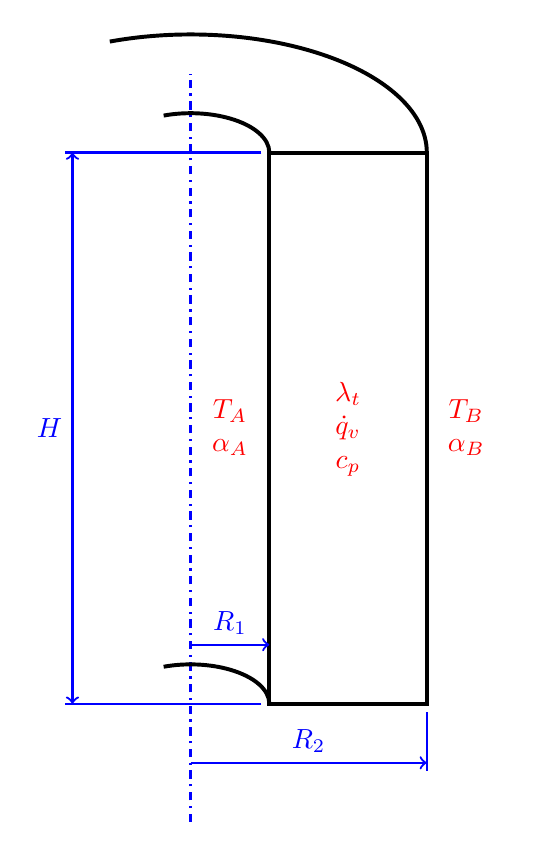
\begin{tikzpicture}
		% Structure
		\draw[black, line width=0.5mm] (1,0) -- ++(2,0) -- ++(0,7) -- ++(-2,0) -- cycle;
		% Eje
		\draw[blue, thick, dashdotted] (0,-1.5) -- ++(0,9.5);
		% Cota H
		\draw[<->, blue, thick] (-1.5,0) -- node[midway, left]{$H$} ++(0,7);
		\draw[blue, thick] (0.9,0) -- ++(-2.5,0);
		\draw[blue, thick] (0.9,7) -- ++(-2.5,0);
		% Cota R1
		\draw[->, blue, thick] (0,0.75) -- node[midway, above]{$R_1$}++(1,0);
		% Cota R2
		\draw[->, blue, thick] (0,-0.75) -- node[midway, above]{$R_2$}++(3,0);
		\draw[blue, thick] (3,-0.85) -- ++(0,0.75);
		% Texto fluido A
		\node[red] at (0.5,3.5) {\begin{tabular}{c} $T_A$ \\ $\alpha_A$ \end{tabular}};
		% Texto fluido B
		\node[red] at (3.5,3.5) {\begin{tabular}{c} $T_B$ \\ $\alpha_B$ \end{tabular}};
		% Texto tubo
		\node[red] at (2,3.5) {\begin{tabular}{c} $\lambda_t$ \\ $\dot{q}_v$ \\ $c_p$ \end{tabular}};
		% Elipses
		\draw[black, line width=0.5mm] (1,0) arc(0:110:1cm and 0.5cm);
		\draw[black, line width=0.5mm] (1,7) arc(0:110:1cm and 0.5cm);
		\draw[black, line width=0.5mm] (3,7) arc(0:110:3cm and 1.5cm);
	\end{tikzpicture}
	\caption{Geometria i propietats termofísiques.}
	\label{fig:plantejament_problema}
\end{figure}

\noindent
Les temperatures dels fluids $A$ i $B$ varien segons les següents lleis:
\begin{align}
	T_A(t) &= T_{A0} + \Delta T_A \, \sin(2 \pi f_A t) \\
	T_B(t) &= T_{B0} + \Delta T_B \, \sin(2 \pi f_B t)
\end{align}
on $T_{A0}$ i $T_{B0}$ són les temperatures mitges, $\Delta T_A$ i $\Delta T_B$ són les amplituds d'oscil·lació, i $f_A$ i $f_B$ són les freqüències d'oscil·lació. 


